\chapter{Optimization: How Networks Learn}\label{ch:optimization}
\begin{center}\small\textit{Knowing the gradient is not enough -- we must walk downhill wisely on a landscape full of valleys and cliffs.}\end{center}

\noindent\fbox{\parbox{\dimexpr\linewidth-2\fboxsep-2\fboxrule}{%
\textbf{From zero: no optimization background assumed.} We start from walking downhill in fog, compare GD, SGD, and mini-batches, and build to momentum, Adam, and schedules. Every formula is preceded by a picture; gradients are defined on first use.}}
\vspace{0.3em}
\section*{Learning Outcomes}
After this chapter you will be able to:
\begin{enumerate}[label=(L\arabic*)]
    \item contrast GD, SGD, and mini-batch updates and their cost trade-offs;
    \item write momentum and Adam updates and explain adaptive steps;
    \item choose learning-rate schedules, warmup, and batch normalization correctly;
    \item tune SGD versus Adam on an example and diagnose common failures.
\end{enumerate}

\section{Intuition: Walking Downhill in Fog}
Imagine a hilly terrain (the loss surface) in thick fog. You can only feel the slope under your feet (the gradient). Stepping opposite to the slope seems wise -- that is \textbf{gradient descent}. But the terrain is high-dimensional, non-convex, and you cannot see far. Steps too small crawl; steps too large overshoot ravines. Mini-batching, momentum, and adaptive steps are tricks for navigating this fog efficiently.

\section{From GD to SGD}
Full gradient descent uses all $n$ examples:
\begin{equation}
\mathbf{w}_{t+1}=\mathbf{w}_t-\eta\,\nabla\mathcal{L}(\mathbf{w}_t),\quad \nabla\mathcal{L}=\frac1n\sum_{i=1}^n\nabla\ell_i(\mathbf{w}_t)
\end{equation}
For ImageNet ($n=1.2$M), one step costs millions of forward passes -- too slow.

\textbf{Stochastic Gradient Descent (SGD)} samples a mini-batch $\mathcal{B}$ of size $B$ (32--256):
\begin{equation}
\mathbf{w}_{t+1}=\mathbf{w}_t-\eta\cdot\frac1B\sum_{i\in\mathcal{B}}\nabla\ell_i(\mathbf{w}_t)
\end{equation}
The mini-batch gradient is noisy but unbiased ($\mathbb{E}[\hat\nabla]=\nabla$). Noise helps escape sharp minima and generalises better.

\begin{definition}[Momentum SGD]
Keep velocity $\mathbf{v}_t$:
\begin{equation}
\mathbf{v}_{t+1}=\mu\mathbf{v}_t+\hat\nabla\mathcal{L}(\mathbf{w}_t),\quad \mathbf{w}_{t+1}=\mathbf{w}_t-\eta\,\mathbf{v}_{t+1}
\end{equation}
Typical $\mu=0.9$. Momentum accelerates along consistent directions and damps oscillation -- like a heavy ball rolling downhill.
\end{definition}

\begin{center}
\begin{tikzpicture}[font=\scriptsize, >=Stealth, scale=0.92]
  % Contour-like loss landscape
  \foreach \r in {0.5,1.0,1.5,2.0} \draw[blue!18, thick] (0,0) ellipse ({\r*1.6} and {\r*0.9});
  \fill[red!70!black] (-2.2,1.2) circle (2pt) node[above left] {start};
  \fill[green!60!black] (0,0) circle (2.5pt) node[below right] {minimum};
  % SGD zigzag
  \draw[->, thick, orange!80!black, decorate, decoration={snake, amplitude=0.3mm, segment length=2mm}] (-2.2,1.2) -- (-1.3,0.8) -- (-0.9,0.2) -- (-0.3,0.1) -- (0,0);
  \node[fill=orange!10, draw=orange!50!black, rounded corners, inner sep=2pt] at (2.2,1.3) {SGD zigzag};
  % Momentum smooth
  \draw[->, thick, violet!80!black] (-2.2,1.2) .. controls (-1.0,1.0) and (-0.6,0.5) .. (0,0);
  \node[fill=violet!10, draw=violet!50!black, rounded corners, inner sep=2pt] at (2.2,0.6) {+momentum};
  \draw[->, thick, gray!60!black] (-2.5,-1.1) -- (-1.2,-1.1) node[midway, above, font=\tiny] {steeper};
  \fill[blue!15] (-2.5,0.8) circle (3pt); \node[right, font=\tiny] at (-2.5,0.8) {contour = equal loss};
\end{tikzpicture}
\end{center}

\section{Adam: Adaptive Moments}
Different parameters need different step sizes (sparse features, ill-conditioning). \textbf{Adam} (Kingma \& Ba, 2015) tracks per-parameter moments:

\begin{equation}
\begin{aligned}
\mathbf{m}_t &= \beta_1\mathbf{m}_{t-1}+(1-\beta_1)\mathbf{g}_t\\
\mathbf{v}_t &= \beta_2\mathbf{v}_{t-1}+(1-\beta_2)\mathbf{g}_t^2\\
\hat{\mathbf{m}}_t&=\mathbf{m}_t/(1-\beta_1^t),\quad \hat{\mathbf{v}}_t=\mathbf{v}_t/(1-\beta_2^t)\\
\mathbf{w}_{t+1}&=\mathbf{w}_t-\eta\,\hat{\mathbf{m}}_t/(\sqrt{\hat{\mathbf{v}}_t}+\epsilon)
\end{aligned}
\end{equation}
Defaults $\beta_1=0.9$, $\beta_2=0.999$, $\epsilon=10^{-8}$, $\eta=10^{-3}$. $\mathbf{m}$ is momentum, $\mathbf{v}$ adapts scale -- parameters with large gradients get smaller effective steps. Bias correction ($\hat{\cdot}$) fixes early-step under-estimate.

\section{Learning Rate Schedules}
A fixed $\eta$ is rarely optimal. Common schedules:
\begin{itemize}
\item \textbf{Step decay:} $\eta_t=\eta_0\cdot\gamma^{\lfloor t/S\rfloor}$ (e.g., halve every 30 epochs).
\item \textbf{Cosine annealing:} $\eta_t=\eta_{\min}+\tfrac12(\eta_{\max}-\eta_{\min})(1+\cos(\pi t/T))$.
\item \textbf{Warmup:} linearly increase from $0$ to $\eta_{\max}$ for first $W$ steps, then decay -- crucial for large batches and Transformers.
\end{itemize}

\begin{center}
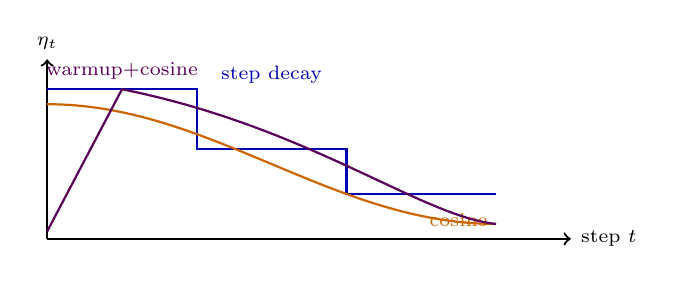
\begin{tikzpicture}[font=\scriptsize, scale=0.95]
  \draw[->, thick] (0,0) -- (7,0) node[right] {step $t$};
  \draw[->, thick] (0,0) -- (0,2.4) node[above] {$\eta_t$};
  % Step decay
  \draw[thick, blue!70!black] (0,2) -- (2,2) -- (2,1.2) -- (4,1.2) -- (4,0.6) -- (6,0.6);
  \node[blue!70!black] at (3,2.2) {step decay};
  % Cosine
  \draw[thick, orange!80!black, domain=0:6, samples=80] plot (\x, {1.0+0.8*cos(180*\x/6)});
  \node[orange!80!black] at (5.5,0.25) {cosine};
  % Warmup
  \draw[thick, violet!70!black] (0,0.1) -- (1,2) -- (1,2) .. controls (3.5,1.5) and (5,0.3) .. (6,0.2);
  \node[violet!70!black] at (1,2.25) {warmup+cosine};
\end{tikzpicture}
\end{center}

\section{Batch Normalization}
Internal covariate shift: as lower layers change, the distribution of inputs to upper layers shifts, forcing them to re-adapt. \textbf{BatchNorm} (Ioffe \& Szegedy, 2015) normalizes each mini-batch:

\begin{equation}
\hat{x}_i=\frac{x_i-\mu_{\mathcal{B}}}{\sqrt{\sigma_{\mathcal{B}}^2+\epsilon}},\qquad y_i=\gamma\hat{x}_i+\beta
\end{equation}
where $\mu_{\mathcal{B}},\sigma_{\mathcal{B}}^2$ are batch mean/variance, $\gamma,\beta$ are learnable scale/shift, and at inference we use running averages. BatchNorm smooths the landscape, allows larger $\eta$, and has a mild regularization effect.

\section{Worked Example: Tuning SGD vs Adam}
\begin{example}[PyTorch-like Training Loop]
\begin{lstlisting}[language=Python]
import torch, math
# Toy: Rosenbrock loss, compare optimizers
def rosenbrock(p): return (1-p[0])**2 + 100*(p[1]-p[0]**2)**2

for name, Opt in [("SGD", torch.optim.SGD), ("Adam", torch.optim.Adam)]:
    p = torch.tensor([0.0, 0.0], requires_grad=True)
    opt = Opt([p], lr=0.01 if name=="Adam" else 0.001, momentum=0.9) if name=="SGD" else Opt([p], lr=0.01)
    sched = torch.optim.lr_scheduler.CosineAnnealingLR(opt, T_max=200)
    for t in range(200):
        opt.zero_grad()
        loss = rosenbrock(p)
        loss.backward()
        # gradient clipping (common with RNNs/Transformers)
        torch.nn.utils.clip_grad_norm_([p], 1.0)
        opt.step(); sched.step()
    print(name, "final", p.detach().numpy(), "loss", loss.item())

# BatchNorm in a linear layer
import torch.nn as nn
layer = nn.Sequential(nn.Linear(64, 64), nn.BatchNorm1d(64), nn.ReLU())
x = torch.randn(32, 64)  # batch of 32
y = layer(x)  # normalized then scaled
print("BN output mean", y.mean().item(), "var", y.var().item())
\end{lstlisting}
\end{example}

\section{Optimization Landscape}
\begin{center}
\begin{tikzpicture}[font=\scriptsize, >=Stealth]
  \node[draw, fill=blue!10, rounded corners, minimum width=2.6cm, minimum height=1.0cm, align=center] (a) at (0,0) {SGD\\{\tiny noisy, good generalizer}};
  \node[draw, fill=green!12, rounded corners, minimum width=2.6cm, minimum height=1.0cm, align=center] (b) at (4,0) {SGD+Momentum\\{\tiny faster, less zigzag}};
  \node[draw, fill=orange!12, rounded corners, minimum width=2.6cm, minimum height=1.0cm, align=center] (c) at (8,0) {Adam\\{\tiny adaptive, fast start}};
  \draw[->, thick, blue!60!black] (a) -- (b) node[midway, above, font=\tiny] {+velocity};
  \draw[->, thick, green!50!black] (b) -- (c) node[midway, above, font=\tiny] {+per-param $\eta$};
  \node[draw, fill=violet!10, rounded corners, font=\tiny, align=center] at (4,-1.5) {All benefit from\\schedules + BatchNorm + clipping};
  \draw[dashed, violet!50!black] (a.south) -- (4,-1.1) -- (c.south);
\end{tikzpicture}
\end{center}

\section{Gradient Noise and Generalization}
Mini-batch noise is not just an artifact -- it acts as implicit regularization.
Small batches find flatter minima (Keskar et al., 2017) that generalize better,
while large batches converge to sharper minima. The noise scale
$g=\eta/B$ predicts this: keep $g$ constant when scaling $B$ and $\eta$.
Second-order methods (Newton, L-BFGS) use curvature but scale poorly to millions
of parameters; diagonal adaptivity (Adam) is the practical compromise.

\section{Weight Initialization Revisited}
Xavier and He initializations were derived to keep $\operatorname{Var}[a^{(l)}]$
constant across layers at initialization. For ReLU, He uses
$W_{ij}\sim\mathcal{N}(0,2/\text{fan}_{in})$. Orthogonal init further helps RNNs.
Poor init makes BatchNorm work harder and can trap optimization in symmetry.

\section{Second-Order Intuition and Limitations}
Newton's step $\mathbf{w}\leftarrow\mathbf{w}-H^{-1}\nabla\mathcal{L}$ uses the
Hessian $H$ to correct for curvature, jumping to the minimum of a quadratic
approximation. But $H$ is $d\times d$ ($d\sim10^7$) -- impossible to store or
invert. Approximations (diagonal, K-FAC, L-BFGS) capture some curvature; Adam's
$\mathbf{v}_t$ is a diagonal Hessian proxy. In practice, well-tuned SGD+momentum
often generalizes slightly better than Adam on vision tasks, while Adam dominates
for Transformers and noisy objectives.

\section{Learning Rate Warmup and Clipping}
Warmup avoids early divergence when gradients are large and Adam's second moment
is uninitialized. Gradient clipping caps $\|\mathbf{g}\|$ to $\tau$ (e.g., 1.0):
if $\|\mathbf{g}\|>\tau$, scale $\mathbf{g}\leftarrow\tau\mathbf{g}/\|\mathbf{g}\|$.
Essential for RNNs/Transformers where backprop through many steps can spike.
Together with cosine decay, warmup+clip is the standard recipe for stable
large-scale training.

\section{Common Pitfalls}
Using Adam with default $\eta=10^{-3}$ on a tiny dataset may overshoot; try
$10^{-4}$ or SGD. Forgetting bias correction in custom Adam causes huge early
steps. Not scheduling $\eta$ wastes 30\% of training time -- a simple cosine
decay is almost free. And never tune on test data: keep a held-out test set
touched once, or your ``improvements'' are illusory.

\section{Further Reading}
Bottou et al. (2018) surveys optimization for ML; Kingma \& Ba (2015) is the
Adam paper; Loshchilov \& Hutter (2019) fixes weight decay. For schedules, see
Loshchilov \& Hutter's \texttt{SGDR} and Smith's cyclical LR. Visualize loss
landscapes with Li et al. (2018) filter-normalized plots -- they explain why
skip connections smooth the terrain.

\section{Chapter Summary}
Optimization navigates a non-convex landscape with noisy gradients. SGD $+$
momentum accelerates; Adam adapts per-parameter steps via $\mathbf{m},\mathbf{v}$.
Schedules (cosine, warmup) and BatchNorm stabilize and accelerate. Gradient
clipping cures explosions; small-batch noise regularizes. No optimizer dominates
universally -- tune $\eta$, $B$, $\lambda$ jointly.

\smallskip
\noindent\textit{Key takeaways:} (1) mini-batch variance $\propto1/B$;
(2) momentum damps zigzag; (3) Adam $=$ momentum $+$ RMS scaling $+$ bias
correction; (4) cosine + warmup is the modern schedule; (5) BatchNorm enables
larger $\eta$ and smoother loss.

\paragraph{Common pitfalls.} Using the same batch statistics at test time, forgetting to shuffle data (correlated batches bias moments), and tuning on the test set are top-3 failures. Always maintain a held-out validation split and fix the random seed for reproducibility.

\begin{example}[Adam step trace] For $g_t=[0.1, -0.2]$, $\beta_1=0.9$, $\beta_2=0.999$, $\epsilon=10^{-8}$, compute $m_1=0.09$, $v_1=0.004$, $\hat m_1=0.09/0.1=0.9$, $\hat v_1=0.004/0.001=4$, update $\Delta=-10^{-3}\cdot0.9/(\sqrt4+10^{-8})\approx-4.5\times10^{-4}$. Small $v$ keeps step moderate; without bias correction, early steps are damped by $1-\beta$.
\end{example}

\section{Exercises}
\begin{exercise} Derive the SGD update variance: if $\operatorname{Var}[\nabla\ell_i]=\sigma^2$, what is $\operatorname{Var}[\hat\nabla_{\mathcal{B}}]$ for batch size $B$? How does $B$ trade noise vs compute?\end{exercise}
\begin{exercise} Adam with $\beta_1=0$ reduces to RMSProp-like scaling. Write the update and explain when momentum helps versus hurts (e.g., ravines vs saddle points).\end{exercise}
\begin{exercise} Implement cosine annealing from scratch and plot $\eta_t$ for $T=100$, $\eta_{\max}=0.1$, $\eta_{\min}=10^{-4}$. Add 10-step linear warmup and show the combined curve.\end{exercise}
\begin{exercise} Explain why BatchNorm uses different statistics at train vs test time. What goes wrong if you use batch statistics at inference with $B=1$?\end{exercise}
\begin{exercise} Train a 3-layer MLP on MNIST with SGD ($\eta=0.1$) and Adam ($\eta=10^{-3}$). Compare loss curves. Now add BatchNorm -- how does the optimal $\eta$ shift?\end{exercise}
% End of Chapter
